%
% budgets.tex
%
% Copyright (C) 2021 by SpaceLab.
%
% FloripaSat-2 Documentation
%
% This work is licensed under the Creative Commons Attribution-ShareAlike 4.0
% International License. To view a copy of this license,
% visit http://creativecommons.org/licenses/by-sa/4.0/.
%

%
% \brief Budgets and mission analysis chapter.
%
% \author Gabriel Mariano Marcelino <gabriel.mm8@gmail.com>
%
% \institution Universidade Federal de Santa Catarina (UFSC)
%
% \version 0.2.0
%
% \date 2020/06/11
%

\chapter{Technical Budgets and Mission Analysis} \label{ch:budgets}

This chapter presents a general analysis of the mission, such as a preliminary analysis of the satellite's estimated orbit, estimated lifetime, and the amount of data exchanged along its operation.

Another type of analysis presented are the satellite budgets, such as the power budget and the link budget.

\section{Orbit Parameters and Analysis}

To define the orbit parameters and simulate the behaviour of the satellite during its operation, the GMAT\nomenclature{\textbf{GMAT}}{\textit{General Mission Analysis Tool.}} software was used \cite{gmat}. The orbit parameters was based on the FloripaSat-I TLE\nomenclature{\textbf{TLE}}{\textit{Two-Line Element.}}, but with a lower altitude. These parameters can be seen in \autoref{tab:orbit-parameters}.

\begin{table}[!h]
    \centering
    \begin{tabular}{lcc}
        \toprule[1.5pt]
        \textbf{Parameters} & \textbf{Value} & \textbf{Unit} \\
        \midrule
        Altitude                & 550           & km \\
        Eccentricity            & 0,0015051     & $^{\circ}$ \\
        Inclination             & 97,9750       & $^{\circ}$ \\
        RAAN                    & 85,5100       & $^{\circ}$ \\
        Arg. of Perigee (AOP)   & 194,87        & $^{\circ}$ \\
        TA                      & 99,8877       & $^{\circ}$ \\
        \bottomrule[1.5pt]
    \end{tabular}
    \caption{Initial orbit parameters (adapted from FloripaSat-I).}
    \label{tab:orbit-parameters}
\end{table}

The parameters of the simulation on GMAT was based on \cite{marino2016} and can be seen below:

\begin{itemize}
    \item Force model for gravitational field: ``\textit{Earth Gravitational Model 1996 (EGM96)}''
    \item Propagator: ``\textit{PrinceDorman78}''
    \item Drag coefficient: 2,2
    \item Drag atmosphere model: ``\textit{Mass Spectrometry and Incoherent Scatter (MSISE90)}''
    \item Epoch: 01 Jan 2022 11:59:28.000
\end{itemize}

The \autoref{fig:fsat2-gmat} shows the 3D representation of the FloripaSat-2 orbit simulation, \autoref{fig:fsat2-gmat-groundtrack} shows the ground track of the first day of operation.

\begin{figure}[!ht]
    \begin{center}
        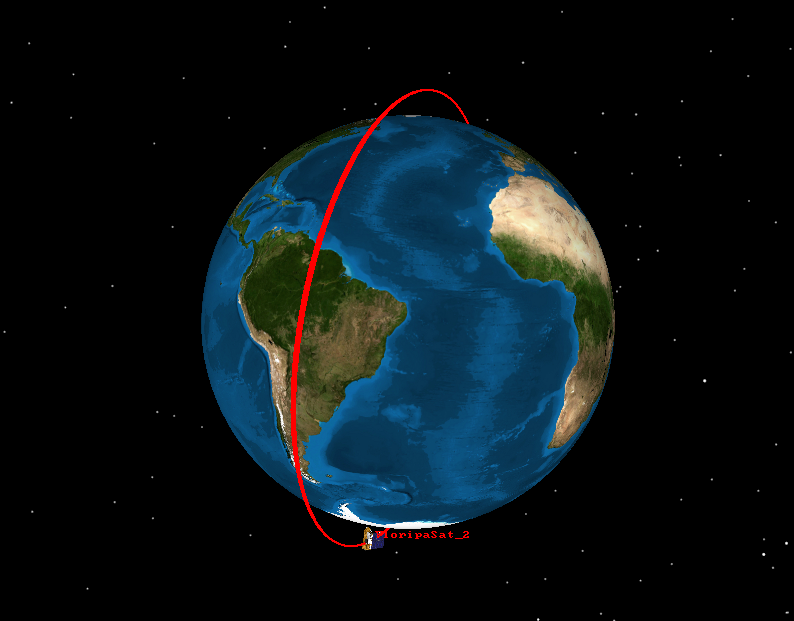
\includegraphics[width=0.6\textwidth]{figures/fsat2-gmat.png}
        \caption{FloripaSat-2 orbit simulation on GMAT.}
        \label{fig:fsat2-gmat}
    \end{center}
\end{figure}

\begin{figure}[!ht]
    \begin{center}
        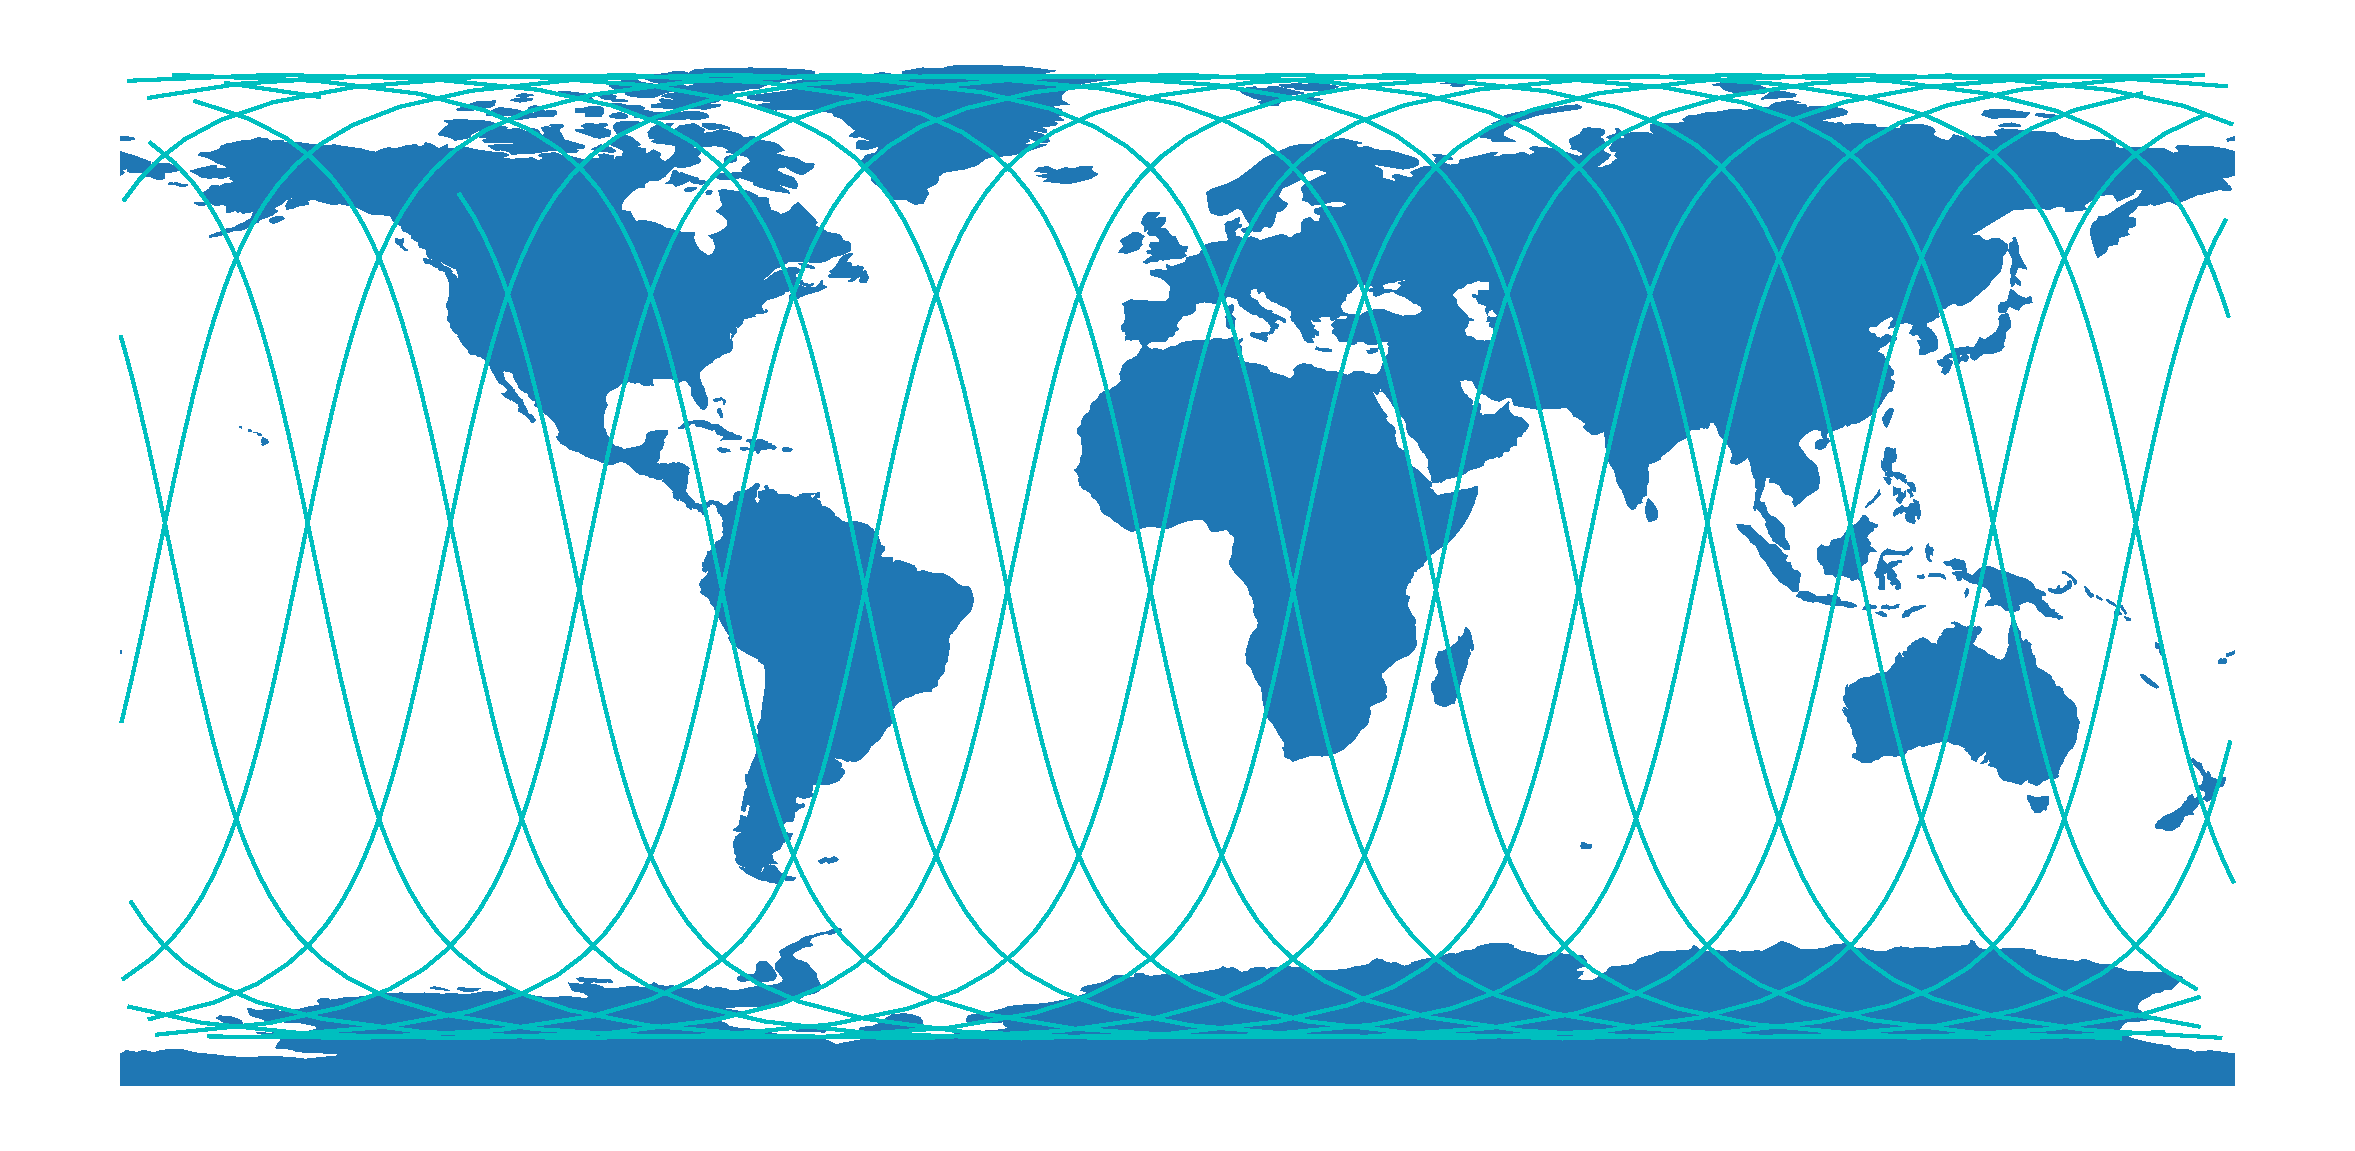
\includegraphics[width=\textwidth]{figures/fsat2-gmat-groundtrack.pdf}
        \caption{FloripaSat-2 simulated groundtrack.}
        \label{fig:fsat2-gmat-groundtrack}
    \end{center}
\end{figure}

The next sections present some analysis based on the results obtained on the simulations executed on GMAT.

The source files of the GMAT simulation are available in \cite{fsat2-mechanical}.

\subsection{Lifetime Analysis}

Considering the same parameters of FloripaSat-I, but with an initial altitude of 550 km, the simulations on GMAT showed that the satellite decays approximately in 2000 days ($\cong$ 5 years), as can be seen in \autoref{fig:lifetime-analysis}.

\begin{figure}[!ht]
    \begin{center}
        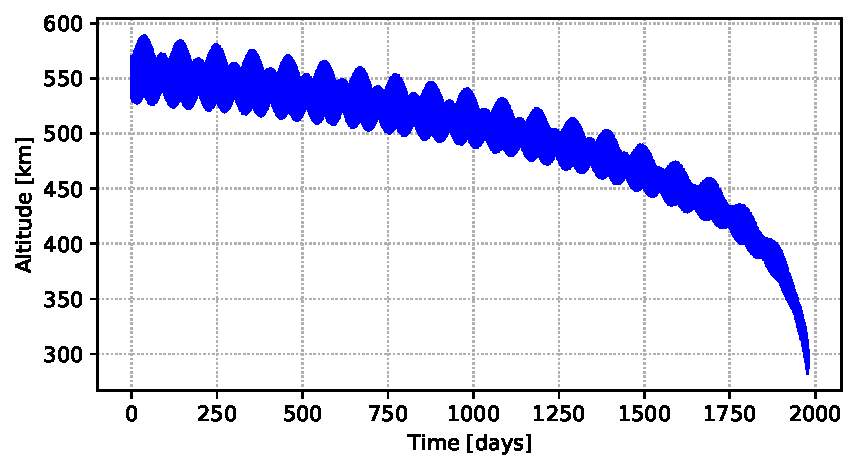
\includegraphics[width=\textwidth]{curves/lifetime.pdf}
        \caption{Lifetime analysis on GMAT.}
        \label{fig:lifetime-analysis}
    \end{center}
\end{figure}

\subsection{Ground Station Passes and Data Transfer Analysis}

Considering two ground stations, one at the SpaceLab installations in Florianópolis (27$^{\circ}$ 36' 00.9" S, 48$^{\circ}$ 31' 03.2" W) and other at the INPE/CRN installations in Natal (5$^{\circ}$ 50' 10.1" S, 35$^{\circ}$ 12' 27.5" W), both with a minimum elevation of 15$^{\circ}$, the following results were achieved during the simulations on GMAT (\autoref{tab:grs-contacts-analysis}).

\begin{table}[!h]
    \centering
    \begin{tabular}{lccc}
        \toprule[1.5pt]
        \textbf{Parameter} & \textbf{UFSC Station} & \textbf{INPE-RN Station} & \textbf{Unit} \\
        \midrule
        Minimum elevation to a valid contact    & 15    & 15    & $^{\circ}$ \\
        Number of contacts                      & 143   & 125   & - \\
        Minimum contact period                  & 24    & 34    & sec \\
        Maximum contact period                  & 395   & 394   & sec \\
        Average contact period                  & 303   & 298   & sec \\
        Total contact period                    & 43394 & 37205 & sec \\
        \bottomrule[1.5pt]
    \end{tabular}
    \caption{Ground station contacts analysis during the first 60 days of operation.}
    \label{tab:grs-contacts-analysis}
\end{table}

As can be seen from \autoref{tab:grs-contacts-analysis}, during the first 60 days of operation, considering the two main ground stations that will contact the satellite, the total contact period is 80599 seconds (43394 + 37205). With the data rate of the downlink/uplink as 4800 bps, this time period will allow a data transfer of 48359400 bytes (or 46,12 M$_{i}$B) between FloripaSat-2 and the Earth. Using the lifetime of the satellite from the previous analysis (2000 days), and an average data transfer per day of 805990 bits, the total theoretical raw data transfer during the whole operation of the satellite will be approximately 1,5 G$_{i}$B.

These values can be even bigger if a smaller minimum elevation is considered, or with more ground stations in other locations.

\section{Mass Budget} \label{mass-budget}

The mass budget of the satellite can be seen in \autoref{tab:mass-budget}.

\begin{table}[!h]
    \centering
    \begin{tabular}{llc}
        \toprule[1.5pt]
        \textbf{Subsystem} & \textbf{Model} & \textbf{Mass [g]} \\
        \midrule
        OBDH            & SpaceLab OBDH 2.0             & TBD \\
        TTC             & SpaceLab TTC 2.0              & TBD \\
        EPS             & SpaceLab EPS 2.0              & TBD \\
        Battery         & SpaceLab Battery Module 4C    & TBD \\
        Antenna         & ISISpace AntS                 & 89 \\
        ACS             & SpaceLab Passive ACS 2U       & TBD \\
        Payload         & INPE-RN EDC                   & TBD \\
        Payload         & SpaceLab Payload X            & TBD \\
        Payload         & SpaceLab Payload Harsh        & TBD \\
        Interface       & SpaceLab Interface Boards     & 40 \\
        Solar Panel     & Orbital Custom Solar Panel    & 266 \\
        Structure       & Usiped Custom 2U Structure    & 206 \\
        Cables          & -                             & TBD \\
        Others          & -                             & TBD \\
        \midrule
        Total           & -                             & \textbf{601} \\
        \bottomrule[1.5pt]
    \end{tabular}
    \caption{Mass budget of the satellite.}
    \label{tab:mass-budget}
\end{table}

According to the CubeSat standard \cite{cds}, the maximum mass of each unit must be 1,33 kg. As the FloripaSat-2 is a 2U CubeSat, the maximum allowed mass of the project is 2,66 kg. Considering the weight of each subsystem presented in \autoref{tab:mass-budget}, the current total mass of the object is below the maximum allowed.

\section{Power Budget} \label{power-budget}

According to section 10.3 of \cite{larson2005}, the power budget of satellite can be determined through three steps:

\begin{enumerate}
    \item Prepare operating power budget
    \item Size the battery
    \item Estimate power degradation over mission life
\end{enumerate}

\subsection{Input Power}

A simulation of the energy input to the solar panels along some orbits can be seen in the \autoref{fig:sp_sim_power} graph. From this simulation, the following results were obtained:

\begin{itemize}
    \item Peak power $\cong$ 8759,5 mW
    \item Average (orbit) $\cong$ 2744,9 mW
    \item Average (sun light) $\cong$ 4315,6 mW
    \item Orbit period $\cong$ 6018 sec
    \item Sun light period $\cong$ 3712 sec
    \item Eclipse period $\cong$ 2124 sec
\end{itemize}

\begin{figure}[!ht]
    \begin{center}
        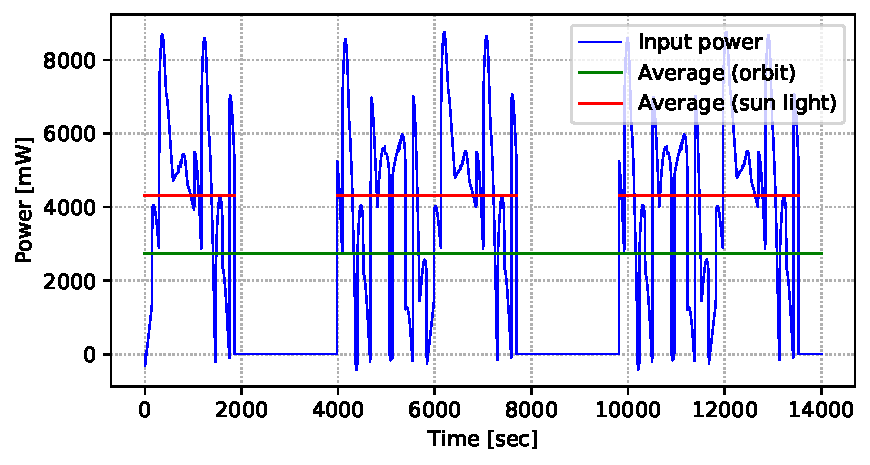
\includegraphics[width=\textwidth]{curves/sp_sim_power}
        \caption{Silumated input power of the solar panels.}
        \label{fig:sp_sim_power}
    \end{center}
\end{figure}

\subsection{Operating Power Budget}

Typical operating voltages, and current and power ranges consumed by each satellite subsystem are presented in \autoref{tab:power-requirements}.

\begin{table}[!h]
    \centering
    \begin{tabular}{lccccc}
        \toprule[1.5pt]
        \multirow{2}{*}{\textbf{Module}} & \multirow{2}{*}{\textbf{Voltage [V]}}    & \multicolumn{2}{c}{\textbf{Current [mA]}} & \multicolumn{2}{c}{\textbf{Power [mW]}} \\
                                         &                                          & \textbf{Min.} & \textbf{Max.}             & \textbf{Min.} & \textbf{Max.} \\
        \midrule
        OBDH                & 3,3   & TBD   & TBD   & TBD   & TBD \\
        TTC ($\mu$C)        & 3,3   & TBD   & TBD   & TBD   & TBD \\
        TTC (radio module)  & 5     & TBD   & 650   & TBD   & 3250 \\
        EPS (digital part)  & 7,4   & TBD   & 40    & TBD   & TBD \\
        EPS (heater)        & 3,3   & TBD   & TBD   & TBD   & TBD \\
        Antenna module      & 3,3   & TBD   & TBD   & TBD   & TBD \\
        Payload EDC         & 5     & 250   & 250   & 1250  & 1250 \\
        Payload-X           & 5     & TBD   & TBD   & TBD   & TBD \\
        Payload Harsh       & 3,3   & TBD   & TBD   & TBD   & TBD \\
        \bottomrule[1.5pt]
    \end{tabular}
    \caption{Power requirements of the subsystems and payloads of the satellite.}
    \label{tab:power-requirements}
\end{table}

Using the information presented in \autoref{tab:power-requirements}, and the activation periods defined for each module, we arrive at the average satellite consumption present in \autoref{tab:power-consumption}.

\begin{table}[!h]
    \centering
    \begin{tabular}{lccccc}
        \toprule[1.5pt]
        \textbf{Module} & \textbf{Duty Cycle [\%]}    & \textbf{Power [mW]} \\
        \midrule
        OBDH                    & 100   & 115 \\
        TTC (radio 1 RX)        & 95    & 65 \\
        TTC (radio 1 TX)        & 5     & 3250 \\
        TTC (radio 2 RX)        & 95    & 65 \\
        TTC (radio 2 TX)        & 5     & 3250 \\
        EPS                     & 100   & 320 \\
        BAT (idle)              & 90    & 0 \\
        BAT (heater full)       & 10    & 5000 \\
        Antenna (deployment)    & 0     & 1800 \\
        Antenna (deployed)      & 100   & 35 \\
        Payload EDC             & 100   & 1250 \\
        Payload Harsh           & 0     & 330 \\
        Payload-X               & 0     & 1000 \\
        \cmidrule{2-3}
                                & \multicolumn{2}{c}{$\cong$ 2668} \\
        \bottomrule[1.5pt]
    \end{tabular}
    \caption{Power consumption of the subsystems and payloads of the satellite.}
    \label{tab:power-consumption}
\end{table}

The duty cycles of \autoref{tab:power-consumption} were defined according to the following assumptions:

\begin{itemize}
    \item One of the EDC payload is always off (cold redundancy).
    \item The Payload-X and the Harsh payload are turned on just during limited periods and only with telecommands.
\end{itemize}

\subsection{Battery Sizing}

\subsection{Power Degradation Over Mission Life}

\begin{itemize}
    \item Solar panels degradation
    \item Battery degradation
\end{itemize}

\section{Link Budget}

The link budget of all radio links of the satellite is available in \autoref{tab:link-budget-results}.

\begin{table}[!h]
    \centering
    \begin{tabular}{L{0.3\textwidth}ccccc}
        \toprule[1.5pt]
        \textbf{Variable} & \textbf{Beacon} & \textbf{Downlink} & \textbf{Uplink} & \textbf{Uplink (Payload)} & \textbf{Unit}\\
        \midrule
        Frequency                       & 437           & 462,5         & 462,5         & 401,635       & MHz \\
        Modulation                      & GMSK          & GMSK          & GMSK          & BPSK          & - \\
        Protocol                        & NGHam         & NGHam         & NGHam         & SBCD          & - \\
        Transmit power                  & 30            & 30            & 47            & 30            & dBm \\
        FSPL                            & 153,9         & 154,4         & 154,4         & 153,2         & dB \\
        Other losses                    & 5             & 5             & 7             & 5             & dB \\
        Transmitter antenna gain        & 0             & 0             & 12            & 3             & dBi \\
        Receiver antenna gain           & 12            & 12            & 0             & 0             & dBi \\
        Receiver noise temp.            & 361,7         & 361,7         & 361,7         & 361,7         & K \\
        Antenna noise temp.             & 300           & 300           & 300           & 300           & K \\
        System noise temp.              & 661,7         & 661,7         & 661,7         & 661,7         & K \\
        Data rate                       & 4800          & 9600          & 9600          & 400           & bps \\
        Received SNR                    & 16,68         & 13,17         & 27,17         & 19,20         & dB \\
        SNR required for $10^{-5}$ BER  & 9,6           & 9,6           & 9,6           & 9,6           & dB \\
        Link margin                     & $\geq$ 7,077  & $\geq$ 3,574  & $\geq$ 17,57  & $\geq$ 9,601  & dB \\
        \bottomrule[1.5pt]
    \end{tabular}
    \caption{Link budget results.}
    \label{tab:link-budget-results}
\end{table}

All equations and steps used to obtain the results of \autoref{tab:link-budget-results} are available in \autoref{anx:link-budget}.
